We call \soset{} the pool of (concrete) solvers we plan to use in parallel to solve a problem. Once we have our solvers set, the last stage is to connect the solvers each others. Up to here, solvers are disconnected, but they have everything to establish the communication. \posl{} provides to the user a platform to easily define cooperative strategies that solvers must follow.

Following, we present two important concepts before we can formalize the {\it communication operators}.

\begin{definition}\label{def:comm_jack}
{\bf (Communication Jack)} Let a solver $\mathcal{S}$ be. Then, the operation $\mathcal{S}\cdot\mathcal{M}$ opens an outgoing connection from the solver $\mathcal{S}$ sending to the outside either 
\begin{inparaenum}[a)]
	\item the output of $\mathcal{M}$ if it is affected by a {\it sending data operator} presented in Definition~\ref{op:osend}, or
	\item $\mathcal{M}$ itself, if it is affected by a {\it sending module operator} presented in Definition~\ref{op:msend}.
\end{inparaenum}
\end{definition} 

\begin{definition}\label{def:comm_outlet}
{\bf (Communication Outlet)} Let a solver $\mathcal{S}$ be. Then, the operation $\mathcal{S}\cdot\mathcal{CM}$ opens an ingoing connection to the solver $\mathcal{S}$ receiving from the outside either 
\begin{inparaenum}[a)]
	\item the output of some \om{} if $\mathcal{CM}$ is a {\it data} \opch{}, or
	\item a \om{} if $\mathcal{CM}$ is an {\it object} \opch.
\end{inparaenum}
\end{definition} 


The communication is established by following the next rules guideline:
\begin{enumerate}%\begin{inparaenum}
	\item Each time a solver sends any kind of information by using a {\it sending} operator, it creates a \jack.
	\item Each time a solver defines a \opch, it creates a \outlet. 
	\item Solvers can be connected each others by linking \jacks{} to \outlets.
\end{enumerate} %\end{inparaenum}

%With the operator $(\cdot)$ we can have access to \oms{} sending information and to the \opch's names in a solver. 
%For example: $Solver_0\cdot \mathcal{M}$ provides access to the \om{} $\mathcal{M}$ in $Solver_0$ if and only if it is affected by a {\it sending} operator, and $Solver_1\cdot CM$ provides access to the \opch{} $CM$ in $Solver_1$.

Following, we define the \textit{connection operators} that \posl{} provides.

\begin{definition}\label{op_conn:1to1}
{\bf (Connection Operator One-to-One)} Let 
\begin{enumerate}
\item the list $\mathcal{J} = \left[\mathcal{S}_0\cdot \mathcal{M}_0, \mathcal{S}_1\cdot \mathcal{M}_1, ..., \mathcal{S}_{N-1}\cdot \mathcal{M}_{N-1}\right]$ of \jacks, and
\item the list $\mathcal{O} = \left[\mathcal{Z}_0\cdot \mathcal{CM}_0, \mathcal{Z}_1\cdot \mathcal{CM}_1, ..., \mathcal{Z}_{N-1}\cdot \mathcal{CM}_{N-1}\right]$ of \outlets{}
\end{enumerate} be. Then, the operation 
\[
\mathcal{J} \poslop{\rightarrow} \mathcal{O}
\]
Connects each \jack{} $\mathcal{S}_i\cdot \mathcal{M}_i \in \mathcal{J}$ with the corresponding \outlet{} $\mathcal{Z}_i\cdot \mathcal{CM}_i \in \mathcal{O}$, $\forall 0 \leq i \leq N-1$.
\end{definition}

\begin{definition}\label{op_conn:1ton}
{\bf (Connection Operator One-to-N)} Let 
\begin{enumerate} 
\item the list $\mathcal{J} = \left[\mathcal{S}_0\cdot \mathcal{M}_0, \mathcal{S}_1\cdot \mathcal{M}_1, ..., \mathcal{S}_{N-1}\cdot \mathcal{M}_{N-1}\right]$ of \jacks, and 
\item the list $\mathcal{O} = \left[\mathcal{Z}_0\cdot \mathcal{CM}_0, \mathcal{Z}_1\cdot \mathcal{CM}_1, ..., \mathcal{Z}_{M-1}\cdot \mathcal{CM}_{M-1}\right]$ of \outlets{} 
\end{enumerate} be. Then, the operation 
\[
\mathcal{J} \poslop{\rightsquigarrow} \mathcal{O}
\]
Connects each \jack{} $\mathcal{S}_i\cdot \mathcal{M}_i \in \mathcal{J}$ with every \outlet{} $\mathcal{Z}_j\cdot \mathcal{CM}_j \in \mathcal{O}$, $\forall 0 \leq i \leq N-1$ and $0 \leq j \leq M-1$.
\end{definition}

\begin{definition}\label{op_conn:ring}
{\bf (Connection Operator Ring)} Let 
\begin{enumerate} 
\item the list $\mathcal{J} = \left[\mathcal{S}_0\cdot \mathcal{M}_0, \mathcal{S}_1\cdot \mathcal{M}_1, ..., \mathcal{S}_{N-1}\cdot \mathcal{M}_{N-1}\right]$ of \jacks, and 
\item the list $\mathcal{O} = \left[\mathcal{S}_0\cdot \mathcal{CM}_0, \mathcal{S}_1\cdot \mathcal{CM}_1, ..., \mathcal{S}_{N-1}\cdot \mathcal{CM}_{N-1}\right]$ of \outlets{} 
\end{enumerate} be. Then, the operation 
\[
\mathcal{J} \poslop{\leftrightarrow} \mathcal{O}
\]
Connects each \jack{} $\mathcal{S}_i\cdot \mathcal{M}_i \in \mathcal{J}$ with the corresponding \outlet{} $\mathcal{Z}_{(i+1)\%N}\cdot \mathcal{CM}_{(i+1)\%N} \in \mathcal{O}$, $\forall 0 \leq i \leq N-1$.
\end{definition}

\begin{figure}[h]
\centering
\subfloat[][Communication 1 to 1]{
	\label{subfig:comm_simple}
	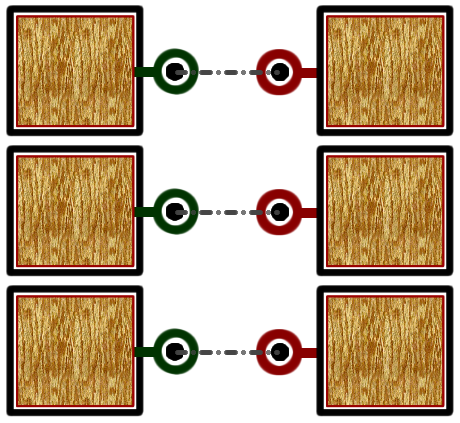
\includegraphics[width=0.25\textwidth]{comm_11.png}
}
\hspace{0.05\textwidth}%
\subfloat[][Communication 1 to N]{%
	\label{subfig:comm_diff}
	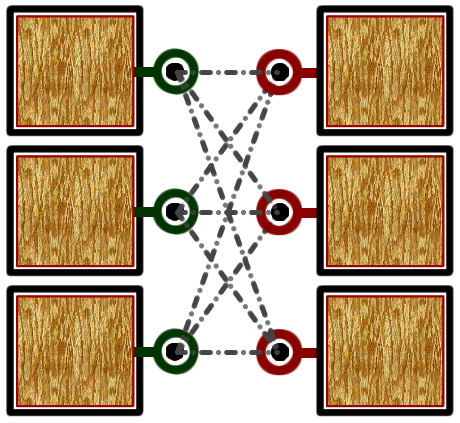
\includegraphics[width=0.25\textwidth]{comm_1n.png}
}
\hspace{0.05\textwidth}%
\subfloat[][Cyclic communication]{%
	\label{subfig:comm_ring}
	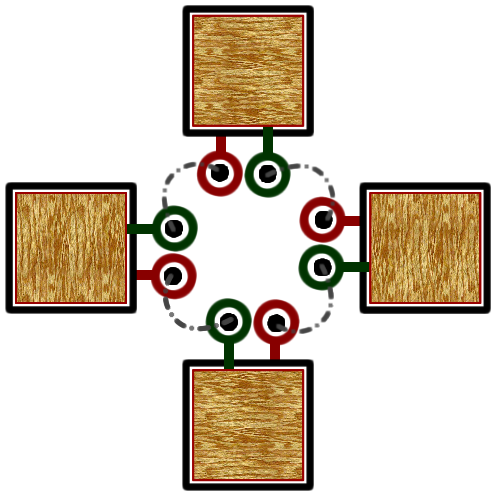
\includegraphics[width=0.25\textwidth]{comm_ring2.png}
}
\caption[]{Graphic representation of communication operators}
\label{fig:comm}
\end{figure}

%These connections \begin{inparaenum}[1.]
%	\item assign an available unit of computation (typically a thread) to each solver, and
%	\item connect solvers each other.
%\end{inparaenum}
 

%We can also schedule non-communicating solvers:
%\[
%\left[\Sigma_0\cdot M_0, \Sigma_1\cdot M_1, ..., \Sigma_{N-1}\cdot M_{N-1}\right]
%\]